\documentclass[12pt,twoside,letterpaper]{article}
%NOTE: This report format is 
\setlength{\footskip}{1.5cm}

\newcommand{\reporttitle}{Procesadores de Lenguajes: Memoria del Proyecto}
\newcommand{\reportauthorOne}{Jose Luis Prado Sierra }
\newcommand{\cidOne}{220070}
\newcommand{\reportauthorTwo}{Alejandro Gragera Serradilla }
\newcommand{\cidTwo}{22M043}
\newcommand{\reportauthorThree}{Antonio Bielza Díez }
\newcommand{\cidThree}{22M049}
\newcommand{\reporttype}{Coursework}

% include files that load packages and define macros
\input{includes} % various packages needed for maths etc.
\input{notation} % short-hand notation and macros


%%%%%%%%%%%%%%%%%%%%%%%%%%%%

\raggedbottom
\begin{document}
% front page
% Last modification: 2016-09-29 (Marc Deisenroth)
% Modification for UW: 2017-05-22 (jphickey)
\begin{titlepage}

\newcommand{\HRule}{\rule{\linewidth}{0.5mm}} % Defines a new command for the horizontal lines, change thickness here


%----------------------------------------------------------------------------------------
%	LOGO SECTION
%----------------------------------------------------------------------------------------



\begin{center} % Center remainder of the page

%----------------------------------------------------------------------------------------
%	HEADING SECTIONS
%----------------------------------------------------------------------------------------

\includegraphics[width = 9cm]{./figures/etsiinf}\\[1.5cm] 
%\textbf{\textsc{\Large Procesadores de Lenguajes}}\\[1.0cm] 
\textsc{\Large Universidad Politécnica de Madrid}\\[0.5cm] 

%----------------------------------------------------------------------------------------
%	TITLE SECTION
%----------------------------------------------------------------------------------------
\vspace{0.75cm}
\HRule \\[0.4cm]
{ \huge \bfseries \reporttitle}\\ % Title of your document
\HRule \\[0.7cm]
    \textsc{\large Analizador Léxico y Tabla de Símbolos}
\end{center}
%----------------------------------------------------------------------------------------
%	AUTHOR SECTION
%----------------------------------------------------------------------------------------

%\begin{minipage}{0.4\hsize}
\vfill
\begin{flushright} \large
    \textsc{\textbf{Grupo 18}}
\\
\reportauthorOne - \cidOne\\ % Your name
\reportauthorTwo - \cidTwo\\ % Your name
\reportauthorThree - \cidThree\\ % Your name
\end{flushright}
%\vspace{4cm}
%\makeatletter
%Date: \@date 

%\vfill % Fill the rest of the page with whitespace



\makeatother


\end{titlepage}




%%%%%%%%%%%%%%%%%%%%%%%%%%% table of content
%If a table of content is needed, simply uncomment the following lines
%\tableofcontents
%\newpage

%%%%%%%%%%%%%%%%%%%%%%%%%%%% Main document
%\section*{Note:}
%\emph{This document is intended to provide a sample structure for the reports in ME303 at the University of Waterloo. }

\section{Analizador Léxico}
%\emph{Describe the physical problem under investigation and the briefly summarize the governing equations. Example:}

Durante el desarrollo del Analizador Léxico hemos descrito una serie de objetos y estructuras matemáticas indispensables para que su diseño, desarrollo y función final cumplan con las expectativas de un Procesador de Lenguajes.

\subsection{Tokens}

Los tokens son duplas que se generan cuando el Analizador Léxico encuentra una concatenación de caracteres que identifica como válida. 
\\
Contienen la información necesaria para que las reciba el Analizador Sintáctico y se componen de un código que los identifica y un atributo opcional que puede servir para diferenciarlos de otros tokens con el mismo código o aportar información extra.
\\
\\
Hemos definido los siguientes tokens en funcion de las necesidades de nuestra práctica:

\begin{itemize}[itemsep=0.1em, topsep=1em, parsep=0pt, partopsep=0pt]
    \item Boolean: $<$BOOLEAN, $>$
    \item Else: $<$ELSE, $>$
    \item Float: $<$FLOAT, $>$
    \item Function: $<$FUNCTION, $>$
    \item If: $<$IF, $>$
    \item Int: $<$INT, $>$
    \item Let: $<$LET, $>$
    \item Read: $<$READ, $>$
    \item Return: $<$RETURN, $>$
    \item String: $<$STRING, $>$
    \item Void: $<$VOID, $>$
    \item Write: $<$WRITE, $>$
    \item Constante real: $<$REALCONST, $>$
    \item Constante entera: $<$INTCONST, $>$
    \item Cadena: $<$STR, "c*"$>$
    \item Identificador: $<$ID, posTS$>$
    \item Suma con asignación (+=): $<$PLUSEQ, $>$
    \item Igual (=): $<$EQ, $>$
    \item Coma (,): $<$COMMA, $>$
    \item Punto y coma (;): $<$SEMICOLON, $>$
    \item Paréntesis abierto ((): $<$OPPAR, $>$
    \item Paréntesis cerrado ()): $<$CLPAR, $>$
    \item Llave abierta (\{): $<$OPBRA, $>$
    \item Llave cerrada (\}:) $<$CLBRA, $>$
    \item Suma (+): $<$SUM, $>$
    \item Y Lógico (\&\&): $<$AND, $>$
    \item Menor ($<$): <MINORTHAN, $>$
    \item false: $<$FALSE, $>$
    \item true: $<$TRUE, $>$
    \item EOF: $<$EOF, $>$
\end{itemize}

Todos los tokens anteriores conforman todos los obligatorios, los específicos y los opcionales de la práctica.

\subsection{Gramática}

La gramática es la estructura matemática que define el lenguaje a generar, en nuestros caso es para una versión reducida de JS. Definir la gramática es una forma de estructurar por tanto el lenguaje y asegurarnos de que vamos a generar solo lo que queremos.
\\
\\
Hemos definido las siguientes reglas:
\begin{itemize}[label={}, itemsep=0.0em, topsep=0.5em]
    \item $S \to ~delS~|~+A~|~\&B~|~`C~|~dD~|~lF~|~\_F~|~/G~|~=~|~,~|~;~|~<~|~(~|~)~|~\{~|~\}$
    \item $A \to ~=~|~\lambda$
    \item $B \to ~\&$
    \item $C \to ~cC~|~`$
    \item $D \to ~dD~|~.E~|~\lambda$
    \item $E \to ~dE~|~d$
    \item $F \to ~lF~|~dF~|~\_F~|~\lambda$
    \item $G \to ~/H$
    \item $H \to ~c_2H~|~\text{\textbackslash n}S$
\end{itemize}
\vspace{1em}
Los conjuntos definidos para el desarrollo de la gramática y del resto de la práctica son: 
\begin{itemize}[label={}, itemsep=0.0em, topsep=0.5em]
    \item Conjunto l: representa cualquier letra.
    \item Conjunto d: representa cualquier dígito.
    \item Conjunto c: representa cualquier caracter.
    \item Conjunto c$_2$: representa cualquier caracter sin \textbackslash n.
\end{itemize}

\subsection{Autómata}

Un autómata es otro tipo de estructura matemática capaz de, al contrario que una gramática que se centra en generar un lenguaje, este se encarga de comprenderlo.
\\
\\
El autómata que hemos planteado capaz de entender todas las palabras válidas de nuestro lenguaje es el siguiente:

\begin{center}
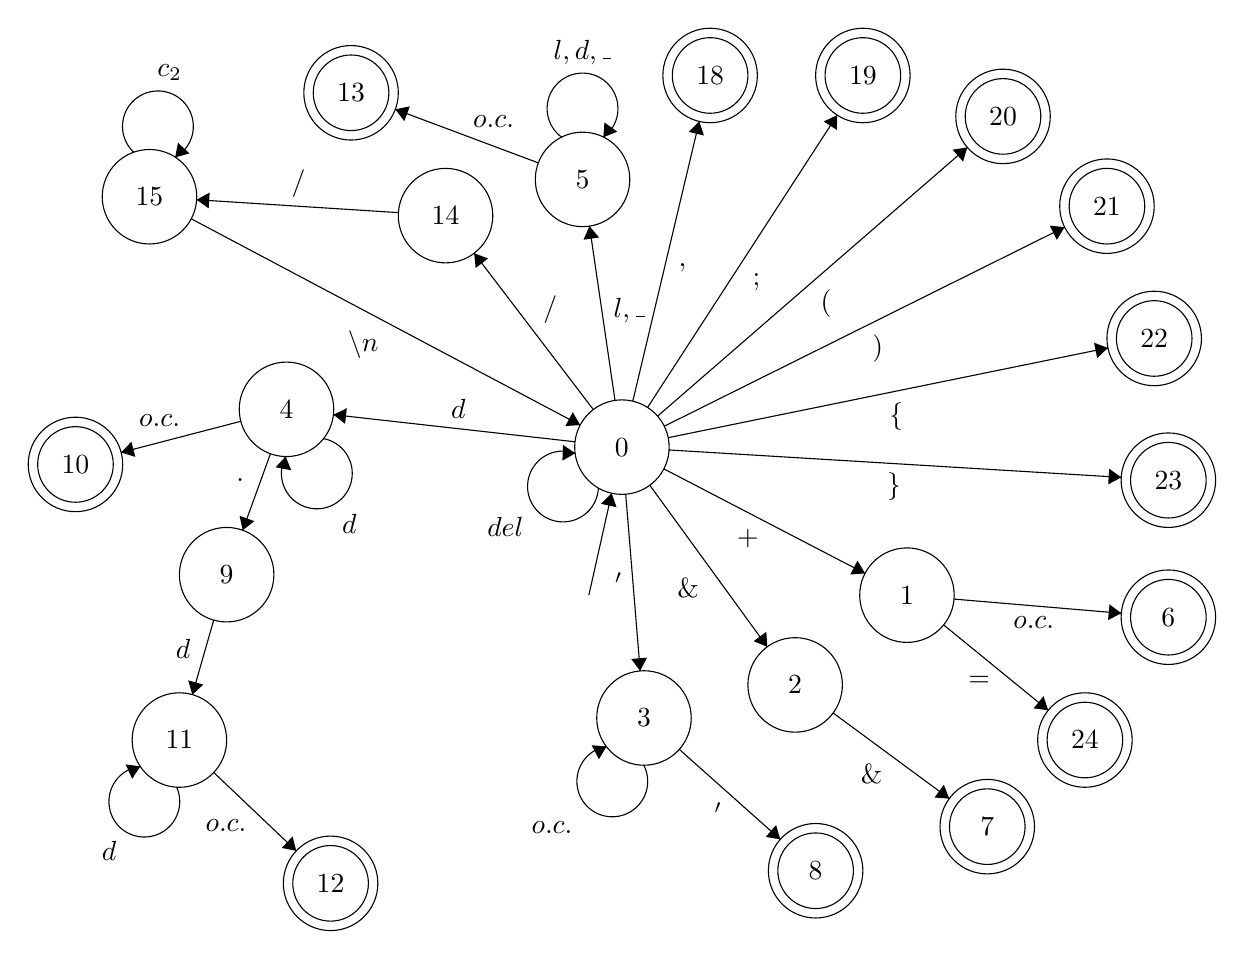
\begin{tikzpicture}[scale=0.2]
\tikzstyle{every node}+=[inner sep=0pt]
\draw [black] (39.8,-27.7) circle (3);
\draw (39.8,-27.7) node {$0$};
\draw [black] (57.9,-37.1) circle (3);
\draw (57.9,-37.1) node {$1$};
\draw [black] (74.5,-38.5) circle (3);
\draw (74.5,-38.5) node {$6$};
\draw [black] (74.5,-38.5) circle (2.4);
\draw [black] (69.2,-46.3) circle (3);
\draw (69.2,-46.3) node {$24$};
\draw [black] (69.2,-46.3) circle (2.4);
\draw [black] (50.8,-42.8) circle (3);
\draw (50.8,-42.8) node {$2$};
\draw [black] (63,-51.8) circle (3);
\draw (63,-51.8) node {$7$};
\draw [black] (63,-51.8) circle (2.4);
\draw [black] (41.2,-44.9) circle (3);
\draw (41.2,-44.9) node {$3$};
\draw [black] (52.1,-54.6) circle (3);
\draw (52.1,-54.6) node {$8$};
\draw [black] (52.1,-54.6) circle (2.4);
\draw [black] (18.5,-25.3) circle (3);
\draw (18.5,-25.3) node {$4$};
\draw [black] (5.1,-28.8) circle (3);
\draw (5.1,-28.8) node {$10$};
\draw [black] (5.1,-28.8) circle (2.4);
\draw [black] (14.7,-35.8) circle (3);
\draw (14.7,-35.8) node {$9$};
\draw [black] (11.7,-46.3) circle (3);
\draw (11.7,-46.3) node {$11$};
\draw [black] (21.3,-55.4) circle (3);
\draw (21.3,-55.4) node {$12$};
\draw [black] (21.3,-55.4) circle (2.4);
\draw [black] (28.6,-13) circle (3);
\draw (28.6,-13) node {$14$};
\draw [black] (9.8,-11.8) circle (3);
\draw (9.8,-11.8) node {$15$};
\draw [black] (37.3,-10.7) circle (3);
\draw (37.3,-10.7) node {$5$};
\draw [black] (22.6,-5.2) circle (3);
\draw (22.6,-5.2) node {$13$};
\draw [black] (22.6,-5.2) circle (2.4);
\draw [black] (45.4,-4.1) circle (3);
\draw (45.4,-4.1) node {$18$};
\draw [black] (45.4,-4.1) circle (2.4);
\draw [black] (55.1,-4.1) circle (3);
\draw (55.1,-4.1) node {$19$};
\draw [black] (55.1,-4.1) circle (2.4);
\draw [black] (64,-6.7) circle (3);
\draw (64,-6.7) node {$20$};
\draw [black] (64,-6.7) circle (2.4);
\draw [black] (70.6,-12.4) circle (3);
\draw (70.6,-12.4) node {$21$};
\draw [black] (70.6,-12.4) circle (2.4);
\draw [black] (73.6,-20.8) circle (3);
\draw (73.6,-20.8) node {$22$};
\draw [black] (73.6,-20.8) circle (2.4);
\draw [black] (74.5,-29.8) circle (3);
\draw (74.5,-29.8) node {$23$};
\draw [black] (74.5,-29.8) circle (2.4);
\draw [black] (38.305,-30.288) arc (-2.28448:-290.28448:2.25);
\draw (33.58,-32.78) node [left] {$del$};
\fill [black] (36.84,-28.09) -- (36.06,-27.56) -- (36.02,-28.56);
\draw [black] (42.46,-29.08) -- (55.24,-35.72);
\fill [black] (55.24,-35.72) -- (54.76,-34.9) -- (54.3,-35.79);
\draw (47.8,-32.9) node [below] {$+$};
\draw [black] (60.23,-38.99) -- (66.87,-44.41);
\fill [black] (66.87,-44.41) -- (66.57,-43.51) -- (65.94,-44.29);
\draw (62.48,-42.19) node [below] {$=$};
\draw [black] (60.89,-37.35) -- (71.51,-38.25);
\fill [black] (71.51,-38.25) -- (70.76,-37.68) -- (70.67,-38.68);
\draw (65.95,-38.43) node [below] {$o.c.$};
\draw [black] (41.57,-30.12) -- (49.03,-40.38);
\fill [black] (49.03,-40.38) -- (48.97,-39.43) -- (48.16,-40.02);
\draw (44.72,-36.63) node [left] {$\&$};
\draw [black] (53.21,-44.58) -- (60.59,-50.02);
\fill [black] (60.59,-50.02) -- (60.24,-49.14) -- (59.65,-49.95);
\draw (55.65,-47.8) node [below] {$\&$};
\draw [black] (40.04,-30.69) -- (40.96,-41.91);
\fill [black] (40.96,-41.91) -- (41.39,-41.07) -- (40.39,-41.15);
\draw (39.88,-36.36) node [left] {$'$};
\draw [black] (41.184,-47.888) arc (27.43495:-260.56505:2.25);
\draw (35.36,-51.45) node [below] {$o.c.$};
\fill [black] (38.82,-46.71) -- (37.88,-46.63) -- (38.34,-47.52);
\draw [black] (43.44,-46.89) -- (49.86,-52.61);
\fill [black] (49.86,-52.61) -- (49.59,-51.7) -- (48.93,-52.45);
\draw (45.92,-50.24) node [below] {$'$};
\draw [black] (36.82,-27.36) -- (21.48,-25.64);
\fill [black] (21.48,-25.64) -- (22.22,-26.22) -- (22.33,-25.23);
\draw (29.41,-25.9) node [above] {$d$};
\draw [black] (20.842,-27.156) arc (79.34618:-208.65382:2.25);
\draw (22.49,-31.91) node [below] {$d$};
\fill [black] (18.45,-28.29) -- (17.81,-28.98) -- (18.8,-29.17);
\draw [black] (15.6,-26.06) -- (8,-28.04);
\fill [black] (8,-28.04) -- (8.9,-28.32) -- (8.65,-27.36);
\draw (10.44,-26.43) node [above] {$o.c.$};
\draw [black] (17.48,-28.12) -- (15.72,-32.98);
\fill [black] (15.72,-32.98) -- (16.46,-32.4) -- (15.52,-32.06);
\draw (15.84,-29.77) node [left] {$.$};
\draw [black] (13.88,-38.68) -- (12.52,-43.42);
\fill [black] (12.52,-43.42) -- (13.22,-42.78) -- (12.26,-42.51);
\draw (12.43,-40.49) node [left] {$d$};
\draw [black] (11.522,-49.283) arc (24.30891:-263.69109:2.25);
\draw (7.24,-52.67) node [below] {$d$};
\fill [black] (9.22,-47.97) -- (8.29,-47.85) -- (8.7,-48.76);
\draw [black] (13.88,-48.36) -- (19.12,-53.34);
\fill [black] (19.12,-53.34) -- (18.89,-52.42) -- (18.2,-53.15);
\draw (14.66,-51.33) node [below] {$o.c.$};
\draw [black] (37.98,-25.31) -- (30.42,-15.39);
\fill [black] (30.42,-15.39) -- (30.51,-16.33) -- (31.3,-15.72);
\draw (34.77,-18.95) node [right] {$/$};
\draw [black] (25.61,-12.81) -- (12.79,-11.99);
\fill [black] (12.79,-11.99) -- (13.56,-12.54) -- (13.62,-11.54);
\draw (19.26,-11.85) node [above] {$/$};
\draw [black] (8.806,-8.982) arc (227.15994:-60.84006:2.25);
\draw (11.08,-4.44) node [above] {$c_2$};
\fill [black] (11.43,-9.3) -- (12.34,-9.05) -- (11.61,-8.37);
\draw [black] (39.36,-24.73) -- (37.74,-13.67);
\fill [black] (37.74,-13.67) -- (37.36,-14.53) -- (38.35,-14.39);
\draw (39.24,-19.02) node [right] {$l,\_$};
\draw [black] (35.977,-8.02) arc (234:-54:2.25);
\draw (37.3,-3.45) node [above] {$l,d,\_$};
\fill [black] (38.62,-8.02) -- (39.5,-7.67) -- (38.69,-7.08);
\draw [black] (34.49,-9.65) -- (25.41,-6.25);
\fill [black] (25.41,-6.25) -- (25.98,-7) -- (26.33,-6.06);
\draw (31.65,-7.41) node [above] {$o.c.$};
\draw [black] (40.49,-24.78) -- (44.71,-7.02);
\fill [black] (44.71,-7.02) -- (44.04,-7.68) -- (45.01,-7.91);
\draw (43.36,-16.32) node [right] {$,$};
\draw [black] (41.43,-25.18) -- (53.47,-6.62);
\fill [black] (53.47,-6.62) -- (52.61,-7.02) -- (53.45,-7.56);
\draw (48.07,-17.22) node [right] {$;$};
\draw [black] (42.07,-25.73) -- (61.73,-8.67);
\fill [black] (61.73,-8.67) -- (60.8,-8.81) -- (61.46,-9.57);
\draw (52.76,-17.69) node [below] {$($};
\draw [black] (42.49,-26.37) -- (67.91,-13.73);
\fill [black] (67.91,-13.73) -- (66.97,-13.64) -- (67.42,-14.54);
\draw (56.04,-20.55) node [below] {$)$};
\draw [black] (42.74,-27.1) -- (70.66,-21.4);
\fill [black] (70.66,-21.4) -- (69.78,-21.07) -- (69.98,-22.05);
\draw (57.23,-24.83) node [below] {$\{$};
\draw [black] (42.79,-27.88) -- (71.51,-29.62);
\fill [black] (71.51,-29.62) -- (70.74,-29.07) -- (70.68,-30.07);
\draw (57.08,-29.3) node [below] {$\}$};
\draw [black] (37.7,-37.1) -- (39.15,-30.63);
\fill [black] (39.15,-30.63) -- (38.48,-31.3) -- (39.46,-31.52);
\draw [black] (12.45,-13.2) -- (37.15,-26.3);
\fill [black] (37.15,-26.3) -- (36.68,-25.48) -- (36.21,-26.36);
\draw (23.37,-20.25) node [below] {$\backslash n$};
\end{tikzpicture}
\end{center}

El autómata tiene que ir acompañado de una serie de acciones que realizar mientras se recorre para poder generar los tokens mientras vamos leyendo el archivo, que vamos a plantear en el siguiente punto.
\\
\\
Cuando aparece una transición o.c. significa que es cualquier otro caracter distinto a las demás transiciones salientes del vértice.

\newpage
\subsection{Acciones Semánticas}

Las acciones semánticas son una serie de acciones que se realizan entre las transiciones del autómata que permiten realizar diferentes funciones como por ejemplo ir generando un string para cuando detectamos una cadena.
\\
\\
Las acciones semánticas que hemos definido para nuestro proyecto son:
\begin{itemize}[label={-}, itemsep=0.0em, topsep=0.5em]
    \item 0:0 Leer
    \item 0:18 Leer, gentoken($<$COMMA, $>$)
    \item 0:19 Leer, gentoken($<$SEMICOLON, $>$)
    \item 0:20 Leer, gentoken($<$OPPAR, $>$)
    \item 0:21 Leer, gentoken($<$CLPAR, $>$)
    \item 0:22 Leer, gentoken($<$OPBRA, $>$)
    \item 0:23 Leer, gentoken($<$CLBRA, $>$)
    \item 0:1 Leer
    \item 1:6 gentoken($<$SUM, $>$)
    \item 1:24 Leer, gentoken($<$EQ, $>$)
    \item 0:2 Leer
    \item 2:7 Leer, gentoken($<$AND, $>$)
    \item 0:3 Leer, $str=''$
    \item 3:3 Leer, $str=str + c$
    \item 3:8 Leer, gentoken($<$STRING, str$>$)
    \item 0:4 Leer, $num=d$
    \item 4:4 Leer, $num = num*10 + d$
    \item 4:10 gentoken($<$INTCONST, num$>$) 
    \item 4:9 Leer, $cont=1$
    \item 9:11 Leer, $num = num*10 + d$, $cont++$
    \item 11:11 Leer, $num = num*10 + d$, $cont++$
    \item 11:12 $num = num*10^{-cont}$, gentoken($<$REALCONST, num$>$)
    \item 0:14 Leer
    \item 0:15 Leer
    \item 15:15 Leer
    \item 15:0 Leer
    \item 0:5 Leer, $id=c$
    \item 5:5 Leer, $id=id + c$
    \item 5:13
    \vspace{-0.2cm}
    \begin{verbatim} 
    if(id in palabrasReservadas)
        posTS = insertTS(id)
        gentoken(<toUpper(id), posTS>)
    else
        posTS = insertTS(id)
        gentoken(<ID, posTS>)
    \end{verbatim}
\end{itemize}


\subsection{Errores}

Todo buen procesador de lenguajes debe de avisar al usuario de si existe algún error y además es capaz de tratar todos los posibles errores para una ejecución robusta y comprensible. 
\\
Sin embargo para esta entrega no es necesario que sean descriptivos pero si han de ser reconocidos y clasificados.
\\
\\
Hemos detectado los siguientes casos capaces de generar errores:
\begin{itemize}[itemsep=0.0em, topsep=0.5em]
    \item \textbf{Cadena mal cerrada:} Al iniciar una cadena si queda mal cerrada (Ej. 'Hola buenas tardes).
    \item \textbf{ID incorrecto:} Al generar o utilizar un ID si los caracteres que lo componen no son correctos.
    \item \textbf{Caracter no reconocido:} Si se recibe un caracter no válido en el estado inicial.
    \item \textbf{Operador lógico incorrecto:} Si se pone un operador lógico (como \&\&) de forma incorrecta (Ej. \&).
    \item \textbf{Comentario de línea mal iniciado:} Al iniciar un comentario de línea incorrectamente (Ej. /Hola buenas tardes).
    \item \textbf{Entero demasiado grande:} Al declarar un entero mayor que 32767.
    \item \textbf{Real demasiado grande:} Al declarar un real mayor que 117549436.
    \item \textbf{Cadena demasiado grande:} Al declarar una cadena de más de 64 caracteres.
\end{itemize}

\newpage
\section{Tabla de Símbolos}

La tabla de símbolos es una estructura de datos que contiene información adicional sobre los tokens cuyo atributo es su posición dentro de ella.
\\
\\
El diseño elegido es una pila de diccionarios en la cual cada diccionario contiene la información extra del token (actualmente vacía) y que, al ser insertados, se devuelve la posición que han recibido dentro de ella, para posteriormente generar el token correctamente.
\\
\\
En nuestro caso se asigna la posición dentro de la tabla de forma lineal, el primer elemento recibe la primera posición y la enésima inserción recibe la enésima posición.

\newpage
\section{Anexo}

\subsection{Casos Correctos}

\subsubsection{Caso Correcto}
\begin{itemize}[label={-}, itemsep=-1em, topsep=0.5em, parsep=-0.2em]
    \item \textbf{Código:}
    \begin{verbatim} 
let int a_53f = 3;
let boolean bb;
let float fl = 3.5;
let int c;
let float fl2;
c = a_53f + 9;
fl2 = fl + 3.0;
let string str = 'Supercalifragilisticoespialidoso';
    \end{verbatim}
    \item \textbf{Archivo de Tokens:}\begin{verbatim}
<LET,>
<INT,>
<ID,0>
<EQ,>
<INTCONST,3>
<SEMICOLON,>
<LET,>
<BOOLEAN,>
<ID,1>
<SEMICOLON,>
<LET,>
<FLOAT,>
<ID,2>
<EQ,>
<REALCONST,3.5>
<SEMICOLON,>
<LET,>
<INT,>
<ID,3>
<SEMICOLON,>
<LET,>
<FLOAT,>
<ID,4>
<SEMICOLON,>
<ID,5>
<EQ,>
<ID,6>
<SUM,>
<INTCONST,9>
<SEMICOLON,>
<ID,7>
<EQ,>
<ID,8>
<SUM,>
<REALCONST,3.0>
<SEMICOLON,>
<LET,>
<STRING,>
<ID,9>
<EQ,>
<STR,"Supercalifragilisticoespialidoso">
<SEMICOLON,>
<EOF,>
    \end{verbatim}
    \item \textbf{Archivo de Tabla de Símbolos:}\begin{verbatim}
CONTENIDOS DE LA TABLA # 1:
* LEXEMA : 'a_53f'
  Atributos:
--------- ---------
* LEXEMA : 'bb'
  Atributos:
--------- ---------
* LEXEMA : 'fl'
  Atributos:
--------- ---------
* LEXEMA : 'c'
  Atributos:
--------- ---------
* LEXEMA : 'fl2'
  Atributos:
--------- ---------
* LEXEMA : 'str'
  Atributos:
--------- ---------
    \end{verbatim}
\end{itemize}

\subsubsection{Caso Correcto}
\begin{itemize}[label={-}, itemsep=-1em, topsep=0.5em, parsep=-0.2em]
    \item \textbf{Código:}
    \begin{verbatim} 
let int s = 2; // Esto es una prueba de comentario 4hjdsh2&&ndj!
s = s + 3; // Sigue siendo una prueba jdlwn;eldr4,4nc,erioe4nx,(·!N$"()E·/$"N
let boolean bs = s && 4;
    \end{verbatim}
    \item \textbf{Archivo de Tokens:}
    \begin{verbatim} 
<LET,>
<INT,>
<ID,0>
<EQ,>
<INTCONST,2>
<SEMICOLON,>
<ID,1>
<EQ,>
<ID,2>
<SUM,>
<INTCONST,3>
<SEMICOLON,>
<LET,>
<BOOLEAN,>
<ID,3>
<EQ,>
<ID,4>
<AND,>
<INTCONST,4>
<SEMICOLON,>
<EOF,>
    \end{verbatim}
    \item \textbf{Archivo de Tabla de Símbolos:}
    \begin{verbatim} 
CONTENIDOS DE LA TABLA # 1:
* LEXEMA : 's'
  Atributos:
--------- ---------
* LEXEMA : 'bs'
  Atributos:
--------- ---------
    \end{verbatim}
\end{itemize}

\newpage
\subsubsection{Caso Correcto}
\begin{itemize}[label={-}, itemsep=-1em, topsep=0.5em, parsep=-0.2em]
    \item \textbf{Código:}
    \begin{verbatim} 
function void sql {
	lt boolean b = true;
		let int dl = 7;
	if (b == true) {
		dl = dl + 2;
		write('Sí');
	}
	else return;
}
    \end{verbatim}
    \item \textbf{Archivo de Tokens:}
    \begin{verbatim} 
<FUNCTION,>
<VOID,>
<ID,0>
<OPBRA,>
<ID,1>
<BOOLEAN,>
<ID,2>
<EQ,>
<TRUE,>
<SEMICOLON,>
<LET,>
<INT,>
<ID,3>
<EQ,>
<INTCONST,7>
<SEMICOLON,>
<IF,>
<OPPAR,>
<ID,4>
<EQ,>
<EQ,>
<TRUE,>
<CLPAR,>
<OPBRA,>
<ID,5>
<EQ,>
<ID,6>
<SUM,>
<INTCONST,2>
<SEMICOLON,>
<WRITE,>
<OPPAR,>
<STR,"Sí">
<CLPAR,>
<SEMICOLON,>
<CLBRA,>
<ELSE,>
<RETURN,>
<SEMICOLON,>
<CLBRA,>
<EOF,>
    \end{verbatim}
    \item \textbf{Archivo de Tabla de Símbolos:}
    \begin{verbatim} 
CONTENIDOS DE LA TABLA # 1:
* LEXEMA : 'sql'
  Atributos:
--------- ---------
* LEXEMA : 'lt'
  Atributos:
--------- ---------
* LEXEMA : 'b'
  Atributos:
--------- ---------
* LEXEMA : 'dl'
  Atributos:
--------- ---------
    \end{verbatim}
\end{itemize}

\newpage
\subsection{Casos Erróneos}
\subsubsection{Caso Erróneo}
\begin{itemize}[label={-}, itemsep=-1em, topsep=0.5em, parsep=-0.2em]
    \item \textbf{Código:}
    \begin{verbatim} 
let int _ser = 45;
let float fl = 564.;
let boolean bl = true;
if (bl & false) int = 3;
    \end{verbatim}
    \item \textbf{Errores:}
    \begin{verbatim} 
Carácter ilegal '.' en línea 2 
Carácter ilegal '&' en línea 4
    \end{verbatim}
\end{itemize}

\subsubsection{Caso Erróneo}
\begin{itemize}[label={-}, itemsep=-1em, topsep=0.5em, parsep=-0.2em]
    \item \textbf{Código:}
    \begin{verbatim} 
let boolean xl3_ = false; / Doremifasollasido
let int del = 3;
del += 4;
if (xl3 == false) write('A'),
    \end{verbatim}
    \item \textbf{Error:}
    \begin{verbatim} 
    Carácter ilegal '/' en línea 1
    \end{verbatim}
\end{itemize}

\subsubsection{Caso Erróneo}
\begin{itemize}[label={-}, itemsep=-1em, topsep=0.0em, parsep=-0.2em]
    \item \textbf{Código:}
    \begin{verbatim} 
let int 3m = 56;
let float ad&d = 3.4;
if (ad&d < 3m) write('Error);
return ad&d;
    \end{verbatim}
    \item \textbf{Errores:}
    \begin{verbatim} 
Carácter ilegal '&' en línea 2
Carácter ilegal '&' en línea 3
Carácter ilegal "'" en línea 3
Carácter ilegal '&' en línea 4
    \end{verbatim}
\end{itemize}


\begin{figure}[h!]
\centering
\includegraphics[width=0.45\textwidth]{figures/goose.png} 
\caption{Ganso intencional.}
\end{figure}

\end{document}
%%% Local Variables: 
%%% mode: latex
%%% TeX-master: t
%%% End: 
